% !TEX program = xelatex
\documentclass[11pt]{article}
\usepackage{graphicx,fontspec,geometry,hyperref,float}
\usepackage[bottom]{footmisc}
\geometry{
	a4paper,
	top=2cm,
	bottom=2cm,
	left=2cm,
	right=2cm
}
% Justify Paragrapher
\newcommand{\justified}
{
	\tolerance=1
	\emergencystretch=\maxdimen
	\hyphenpenalty=10000
	\hbadness=10000
}


\graphicspath{ {./images/} }
\setmainfont{Times New Roman}

\title{
	\vspace{-2cm}
	\textbf{Artificial Neural Network and Deep Learning}\\
	\large Homework 1
}
\date{}

\author{Angelo Capponcelli \and Pasquale Castiglione \and Mehdi Samimi}

\begin{document}
\maketitle
\justified

\section*{Data Load and Augmentation}
In order to estimate the model's capabilities and tweaking the hyperparameters consequently, we have split the data in training-set and validation-set. During the development a ratio of 80/20 turned out to be the best choice for the splitting.\\
Because of the relative small amount of training data, \emph{image augmentation} was performed. In particular, given the nature of the training images, we considered worthwhile to apply \textbf{Random Flip}, \textbf{Random Rotation}, \textbf{Random Brightness Adjustment}, \textbf{Random Zoom} and \textbf{Random Shift} since, all these operations wouldn't have changed the meaning of the data regarding this classification task.\\
During development, we also tried, to use \emph{Oversampling} and \emph{Downsampling} in order to try to solve the problem of class imbalance by equaling the number of samples for each class but this led to no improvement in the result.\\
For the models that used Transfer Learning a  \textbf{preprocess\_function} was also used.

\begin{figure}[H]
\center
	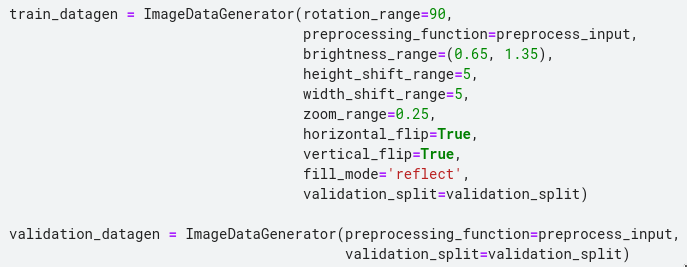
\includegraphics[scale=0.4]{imageDataGenerator.png}
	\caption{ImageDataGenerators}
\end{figure}

\section*{First Approach}
The first model developed was a simply CNN with four convolutional blocks.\\ Each block was composed of one convolutional layer with a 3x3 filter, a \emph{ReLu} activation function and a \emph{MaxPooling} layer. The number of filters of the convolutional layers went from 32 in the first block to 256 in the last, doubling it in each block. For the fully connected part we tried with both 256 and 512 neurons, experimenting with different number of hidden layers. But, at the end, just a single hidden layer with 256 neurons showed the best result.\\
Between the convolutional part and the fully connected part we used a \emph{Global Average Pooling} layer instead of a \emph{Flatten} layer in order to improve the generalization capabilities of the model.\\
This first approach lead us to an initial accuracy of $\approx0.60$ and, by adding \emph{BatchNormalization} layers and tweaking the parameters, we've managed to reach firstly an accuracy of $\approx0.70$ and, in the end, an accuracy of $\approx0.77$ with both the provided and the complete dataset.

\begin{figure}[H]
	\center
	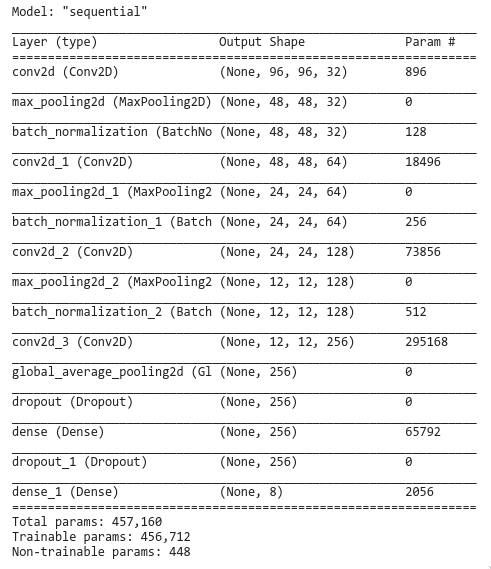
\includegraphics[scale=0.35]{model1.png}
	\caption{One of the model of the First Approach}
\end{figure}

\begin{figure}[H]
	\center
	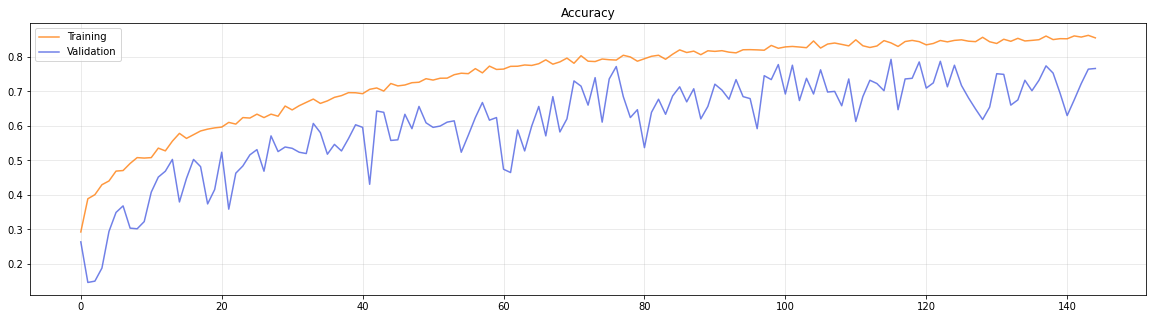
\includegraphics[width=\textwidth]{first_model_accuracy.png}
	\caption{Accuracy in the first approach}
\end{figure}



\section*{Transfer Learning}
Getting no more substantial improvements, we decided to change strategy and perform \emph{Transfer Learning}. After experimenting with \emph{VGG16\footnote{\url{https://arxiv.org/abs/1409.1556}}}, which lead us to an accuracy score of $\approx0.81$, we went with \emph{Inception\_V3\footnote{\url{https://arxiv.org/abs/1512.00567}}}.\\
We imported only the feature extraction layers and added a simple fully connected part, which, at the end, consisted of two hidden dense layers of 256 neurons each and a final output layer. \emph{Dropout} layers were used in between the dense layers in order to reduce overfitting. Input shape was set to (139,139,3).\footnote{During development, we wrongly read that for inceptionV3 ``width and height should be no smaller than 139'' but, actually, the keras documentation says ``width and height should be no smaller than 75''. However (139,139,3) gave us better results}\\
The training consisted of three, consequent, phases:
\begin{itemize}
	\item \textbf{Transfer Learning}: In this phase we froze the first 288 layers of the model in order to have a rough initialization of the dense layers and so we trained the model with ADAM's default learning rate. In this phase accuracy reached $\approx0.70$. In the beginning we froze all the layers as seen during the labs, but allowing some of last layers to be trained gave us better results.
	\item \textbf{Partial Fine Tuning}: At this point we unfreeze the layers up to the 215th one, we reduced the learning rate to 8e-4 and retrained the model for less epochs. Accuracy, at this point, reached $\approx0.75$.
	\item \textbf{Full Fine Tuning}: In this last part we unfreezed the entire model and reduced the optimizer's learning rate to 1e-5 in order to just adapt the pretrained features to the specific task and avoid too much overfitting. We were able to get an accuracy of $\approx0.84$ 
\end{itemize}
During all this three training  phases \emph{Early stopping} on validation loss was used in order to prevent overfitting and to reduce the training time.\\
Since the dataset was imbalanced, we also used the \emph{class\_weight} attribute to try to solve this problem but this didn't give us the desired outcome.\\
This model turned out to be pretty much robust during both Development and Final phase of the competition achieving the same performance.

\begin{figure}[H]
	\center
	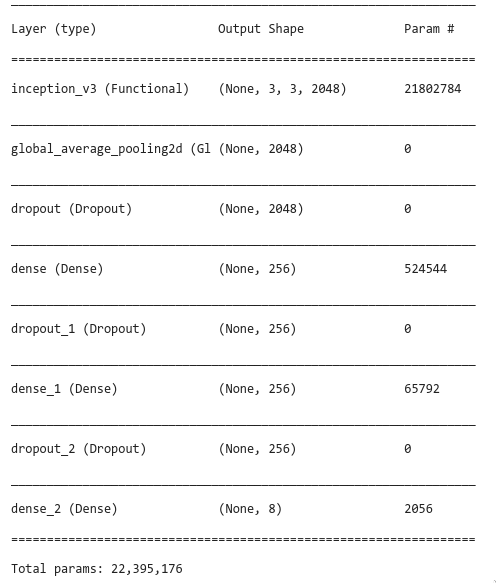
\includegraphics[scale=0.35]{final_summary.png}
	\caption{Summary of the Final Model}
\end{figure}

\begin{figure}[H]
	\center
	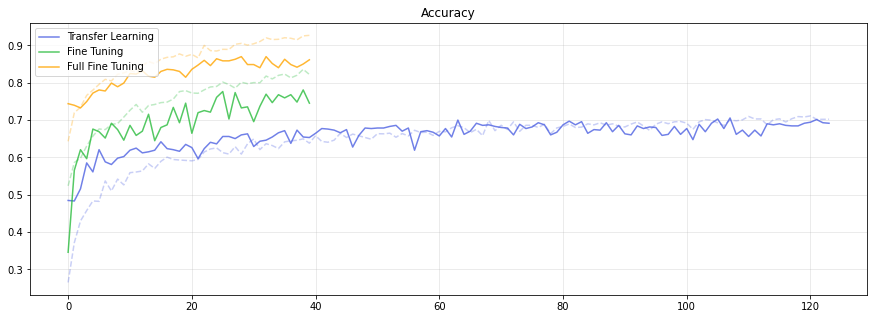
\includegraphics[width=\textwidth]{final_model_accuracy.png}
	\caption{Accuracy of the Final Model}
\end{figure}

\section*{Conclusion}
For the development we mainly use Kaggle in order to take advantage of the free GPU power and so to reduce the training time.\\
In order to analyze the models and take decisions accordingly, we used the plots of the accuracy and the loss over the epochs to understand better what was going on.
\end{document}
